\chapter{Sistem Indra}\label{ch:b3:sensory-systems}

Pada malam yang gelap sebuah mata manusia dapat mendeteksi sebuah kilatan
beberapa foton --- yakni jumlah cahaya terkecil yang diizinkan fisika untuk
dideteksi sama sekali. Telinganya mendengar sebuah bunyi yang menggerakkan
gendang telinganya kurang daripada garis tengah sebuah atom hidrogen, lalu
membedakan sebuah nada dari nada lain yang berbeda seperlima persen. Seekor
anjing mengikuti sebuah jejak berisi beberapa molekul tiap sentimeter kubik;
seekor hiu menemukan seekor ikan sebelah di bawah pasir lewat medan listrik
detak jantungnya. Tiap indra bermula dengan sebuah sel yang mengubah satu jenis
tenaga menjadi sebuah perubahan potensial selaput, dan tiap indra berakhir
sebagai lecutan di dalam sebuah saraf; di antara keduanya terletak masalah
yang diperlakukan bab ini: bagaimana sebuah reseptor melipatgandakan sebuah
molekul atau foton tunggal menjadi sebuah isyarat yang dapat dibaca neuron,
bagaimana sebuah jangkauan sejuta juta kali lipat dalam keamatan diperas menjadi
sebuah laju beberapa ratus lecutan tiap detik, bagaimana sebuah gelombang mekanis
disortir menurut frekuensinya, bagaimana sepuluh ribu bau dibedakan dengan empat
ratus reseptor, dan bagaimana otaknya, yang tidak pernah menerima apa pun selain
lecutan, tahu dari indra mana lecutan itu datang.

\section{Asas yang sama pada tiap indra}

\begin{definition}[Transduksi, penyandian, dan adaptasi]\label{def:b3:sensory-systems:principles}
\index{transduksi indra}\index{potensial reseptor}\index{jalur berlabel}%
\index{medan reseptif}\index{adaptasi!indra}\index{penghambatan lateral}
Sebuah \emph{sel reseptor indra} memuat sebuah mekanisme \emph{transduksi}
--- sebuah protein atau runtunan --- yang mengubah sebuah rangsang (sebuah foton,
sebuah molekul, sebuah pergeseran, panas, sebuah medan listrik) menjadi sebuah
perubahan kehantaran selaput sehingga menjadi sebuah \emph{potensial reseptor},
yang berjenjang dengan rangsangnya; selnya, atau neuron yang disinapsisinya,
mengubah ini menjadi sebuah deretan potensial aksi yang lajunya menyandi
keamatannya. \emph{Modalitas} sebuah isyarat diberikan bukan oleh lecutannya,
yang serupa pada tiap saraf, melainkan oleh kawat yang dilaluinya dan tempat
kawat itu berakhir di dalam otaknya: itulah sebuah \emph{jalur berlabel}. Sebuah
neuron indra menanggapi rangsang di dalam sebuah \emph{medan reseptif} --- sepetak
kulit, sebuah daerah medan penglihatan, sebuah pita frekuensi --- dan medan yang
bertetangga saling menajamkan lewat \emph{penghambatan lateral}, dengan tiap
neuron menekan tetangganya sehingga tepi dan kontrasnya dilebih-lebihkan.
Kebanyakan reseptor \emph{beradaptasi}: tanggapannya terhadap rangsang yang
dipertahankan menurun, sehingga mereka melaporkan perubahan alih-alih arasnya,
dan jangkauan kerjanya bergeser untuk duduk di sekitar latar yang berlaku.
\end{definition}

\begin{theorem}[Weber, Fechner, dan Stevens]\label{thm:b3:sensory-systems:weber}
\index{hukum Weber}\index{hukum Fechner}\index{hukum pangkat Stevens}
Pengamatan Weber (1834) adalah bahwa perubahan terkecil yang terdeteksi
$\Delta I$ pada sebuah rangsang berkeamatan $I$ adalah sebuah pecahan tetap
darinya: $\Delta I/I = k$, dengan $k$ sekitar $0.02$ bagi bobot, $0.08$ bagi
kecerahan, $0.1$ bagi kenyaringan. Bila tiap beda yang baru terasa
dihitung sebagai satu satuan penginderaan $S$, maka $\mathrm{d}S = \mathrm{d}I/
(kI)$ dan
\[
S = \frac{1}{k}\ln\frac{I}{I_{0}} ,
\]
dengan $I_{0}$ adalah ambangnya: penginderaannya tumbuh sebagai logaritma
rangsangnya (Fechner, 1860), dan itulah sebabnya keamatan diukur dalam
\omterm{def:b3:sensory-systems:cochlea}{desibel} dan magnitudo, serta sebabnya sebatang lilin yang ditambahkan kepada
sebatang lilin terperhatikan sementara sebatang lilin yang ditambahkan kepada
sebuah lampu sorot tidak. Percobaan penskalaan langsung, yang di dalamnya
subjek memberikan angka kepada penginderaannya, justru memberi sebuah hukum
pangkat $S \propto I^{n}$ (Stevens, 1957), dengan $n \approx
0.3$ bagi kenyaringan dan kecerahan, $1$ bagi panjang garis, dan $3.5$ bagi
sengatan listrik; sebuah logaritma dan sebuah pangkat kecil nyaris tak
terbedakan sepanjang beberapa dasawarsa, dan kedua hukumnya sepakat pada
pokoknya: sistem sarafnya memampatkan.
\end{theorem}
\begin{proof}
Dari $\Delta I = kI$ bagi satu satuan $S$, pertambahan penginderaannya
tiap pertambahan rangsangnya adalah $\mathrm{d}S/\mathrm{d}I = 1/(kI)$;
dengan mengintegralkannya dari ambangnya $I_{0}$, tempat $S = 0$, diperoleh $S = (1/k)
\ln(I/I_{0})$. Hukum pangkatnya adalah anggapan alternatif bahwa sebuah
\emph{nisbah} rangsang yang tetap menghasilkan sebuah \emph{nisbah} penginderaan yang tetap,
$\mathrm{d}S/S = n\,\mathrm{d}I/I$, yang integralnya adalah $S \propto I^{n}$;
bagi $n \to 0$ dengan penskalaan yang sesuai ia menuju logaritmanya.
\end{proof}

\begin{omfigure}
\begin{tikzpicture}
\begin{axis}[
  width=0.68\linewidth, height=5.6cm,
  xmode=log,
  xmin=1, xmax=1e6, ymin=0, ymax=15,
  xlabel={keamatan rangsang $I/I_{0}$}, ylabel={penginderaan $S$ (sebarang)},
  xlabel style={font=\small, at={(axis description cs:0.5,-0.12)}, anchor=north}, ylabel style={font=\small},
  tick label style={font=\small}, ytick={0,5,10,15},
  clip=false,
]
\addplot[very thick, omDef, domain=1:1e6, samples=100] {ln(x)};
\addplot[very thick, omThm, domain=1:1e6, samples=100] {0.235*x^0.3 - 0.235};
\addplot[very thick, omMeth!70!black, domain=1:1e6, samples=100] {0.5*x^0.24 - 0.5};
\node[font=\scriptsize, omDef, anchor=north west] at (axis cs:2,10.2) {Fechner: $S = \ln(I/I_{0})$};
\node[font=\scriptsize, omThm, anchor=south east] at (axis cs:9e5,0.4) {Stevens: $S \propto I^{0.3}$};
\node[font=\scriptsize, omMeth!70!black, anchor=north west] at (axis cs:2,12.5) {Stevens: $S \propto I^{0.24}$};
\end{axis}
\end{tikzpicture}

{\small Pemampatan sebuah jangkauan keamatan sejuta kali lipat menjadi sebuah
penginderaan yang tumbuh lambat: logaritma Fechner dan \omterm{thm:b3:sensory-systems:weber}{hukum pangkat Stevens}
dengan pangkat yang kecil sukar dibedakan sepanjang beberapa dasawarsa, dan
keduanya mengatakan bahwa indranya melaporkan nisbah, bukan selisih.}
\end{omfigure}

\section{Penglihatan}

\begin{definition}[Retina]\label{def:b3:sensory-systems:retina}
\index{retina}\index{sel batang}\index{sel kerucut}\index{fototransduksi}%
\index{rodopsin}\index{sel ganglion}\index{pusat--sekeliling}
\emph{Retina} adalah selembar otak di belakang mata, tiga
lapis sel dengan fotoreseptornya, yang secara paradoks, di belakang,
menempel pada epitelium pigmennya. \emph{Sel batang} --- $10^{8}$ tiap mata, satu
pigmen, \emph{rodopsin} --- melayani cahaya redup lalu menjenuh pada siang hari;
\emph{sel kerucut} --- $6\times 10^{6}$, tiga pigmen yang memuncak pada biru,
hijau, dan merah, yang terkemas ke dalam fovea --- melayani siang hari, warna, dan
ketajaman. \emph{Fototransduksi} adalah sebuah runtunan: sebuah foton
mengisomerkan kromofor retinal satu rodopsin; rodopsin yang teraktif menyalakan
ratusan molekul protein~G transdusin, yang masing-masing
mengaktifkan sebuah fosfodiesterase yang memusnahkan GMP siklik; turunnya
cGMP menutup saluran kation yang ditahan cGMP tetap terbuka di dalam gelap,
``arus gelap'' yang masuk berhenti, dan selnya \emph{terhiperpolarisasi} ---
cahaya mematikan sebuah fotoreseptor, dan ia melepaskan lebih sedikit glutamat. Di dalam
gelap selnya terdepolarisasi lalu melepaskan terus-menerus. Isyaratnya
lewat ke \emph{sel bipolar} (berjenis ON dan OFF, yang membalikkan atau
mempertahankannya) lalu ke \emph{sel \omterm{def:b3:nervous-systems:comparative}{ganglion}}, sejuta tiap mata,
yang aksonnya membentuk saraf optiknya --- sebuah pemampatan seratus kali lipat.
Sel horizontal dan amakrin menyambung secara lateral, dan penghambatannya
memberi tiap sel \omterm{def:b3:nervous-systems:comparative}{ganglion} sebuah \omterm{def:b3:sensory-systems:principles}{medan reseptif} \emph{pusat--sekeliling}:
terpacu oleh cahaya pada sebuah cakram pusat dan terhambat oleh cahaya pada cincin
di sekitarnya (atau sebaliknya), sehingga retinanya melaporkan kontras setempat
dan tepi alih-alih cahaya mutlak.
\end{definition}

\begin{omfigure}
\begin{tikzpicture}[every node/.style={font=\scriptsize}, >=stealth]
  % cascade boxes with amplification numbers
  \node[draw, thick, rounded corners, fill=omProp!30, align=center] (ph) at (0,0) {1 foton};
  \node[draw, thick, rounded corners, fill=omDef!20, align=center] (rh) at (2.6,0) {1 rodopsin*\\(metarodopsin II)};
  \node[draw, thick, rounded corners, fill=omDef!20, align=center] (tr) at (5.6,0) {$\sim 500$ transdusin\\teraktifkan};
  \node[draw, thick, rounded corners, fill=omDef!20, align=center] (pde) at (8.6,0) {$\sim 500$ PDE aktif:\\$\sim 10^{5}$ cGMP terhidrolisis};
  \node[draw, thick, rounded corners, fill=omThm!20, align=center] (ch) at (5.6,-2.0) {$\sim 200$ saluran kation menutup;\\arus gelapnya turun \qty{1}{pA}};
  \node[draw, thick, rounded corners, fill=omMeth!25, align=center] (out) at (1.4,-2.0) {hiperpolarisasi \qty{1}{mV};\\glutamat yang dilepaskan berkurang};
  \draw[->, thick] (ph) -- (rh); \draw[->, thick] (rh) -- (tr); \draw[->, thick] (tr) -- (pde);
  \draw[->, thick] (pde.south) |- (ch.east); \draw[->, thick] (ch) -- (out);
  \node[below, font=\tiny, align=center] at (7.1,-2.8) {tiap langkah mengalikan; seluruh runtunannya dimatikan dalam \qty{200}{ms} oleh\\kinase rodopsin, arestin, dan GTPase transdusin, lalu disetel ulang};
\end{tikzpicture}

{\small \omterm{def:b3:sensory-systems:retina}{Fototransduksi} sebagai sebuah pelipat ganda. Satu foton yang diserap
menutup ratusan saluran lewat dua tahap katalitik, yakni sebuah bati sekitar
sejuta dalam molekul --- cukup bagi satu foton untuk menghasilkan sebuah arus
yang terukur di dalam sebuah \omterm{def:b3:sensory-systems:retina}{sel batang}.}
\end{omfigure}

\begin{theorem}[Mencacah foton: kekerapan melihat]\label{thm:b3:sensory-systems:hecht}
\index{pendeteksian foton tunggal}\index{kurva kekerapan melihat}%
\index{Poisson!pencacahan foton}
Sebuah kilatan yang menghantarkan rata-rata $a$ foton terserap ke sepetak
\omterm{def:b3:sensory-systems:retina}{sel batang} menghantarkan, pada sembarang satu penyajian, sebuah cacah $k$ yang
tersebar Poisson: $P(k) = e^{-a}a^{k}/k!$. Bila pengamatnya melaporkan melihat
kilatannya kapan pun sedikitnya $n$ foton terserap, peluang
melihatnya adalah
\[
P_{\text{lihat}}(a) = 1 - \sum_{k=0}^{n-1} e^{-a}\,\frac{a^{k}}{k!} ,
\]
yakni sebuah kurva yang naik dari $0$ ke $1$ seiring naiknya $a$, dan yang
\emph{kecuramannya} pada skala logaritma $a$ bergantung hanya pada $n$:
makin besar cacah ambangnya, makin curam kurvanya. Mencocokkan
\omterm{thm:b3:sensory-systems:hecht}{kurva kekerapan melihat} yang terukur karena itu memberi $n$ tanpa
mengetahui berapa banyak foton yang dihantarkan yang benar-benar terserap.
\end{theorem}
\begin{proof}
Foton dari sebuah sumber lemah yang tetap tiba secara bebas dan acak, dan
cacah yang terserap dalam sebuah kilatan pendek dari sebuah rata-rata $a$ bersebaran Poisson
(yakni limit sebuah binomial dengan banyak foton yang masing-masing terserap dengan peluang
kecil). Melihat menuntut $k \ge n$, yang peluangnya adalah satu
dikurangi jumlah $n$ suku Poisson yang pertama. Menskalakan sumbernya dengan sebuah
faktor $c$ mengalikan $a$ dengan $c$ lalu menggeser kurvanya sepanjang sumbu $\log a$
tanpa mengubah bentuknya, sehingga bentuknya mengenali $n$: bagi $n =
1$, $P = 1 - e^{-a}$ naik sepanjang dua dasawarsa $a$; bagi $n = 6$ ia
naik sepanjang kurang daripada satu.
\end{proof}

\begin{proof}[Bukti eksperimental]
Hecht, Shlaer, dan Pirenne (1942) mendudukkan pengamat di dalam gelap selama
setengah jam, lalu mengilatkan sebuah bintik hijau mungil pada tepi \omterm{def:b3:sensory-systems:retina}{retinanya}
yang kaya \omterm{def:b3:sensory-systems:retina}{sel batang} selama semilidetik, ratusan kali pada beberapa keamatan,
lalu mencatat bagian kilatan yang terlihat. Kilatan ambangnya
memuat, pada korneanya, sekitar $90$ foton, yang darinya (sesudah
pemantulan, penyerapan di dalam media matanya, dan peluang $20\,\%$ sebuah
foton yang mencapai sebuah \omterm{def:b3:sensory-systems:retina}{sel batang} untuk diserap \omterm{def:b3:sensory-systems:retina}{rodopsin}) sekitar $5$--$14$
terserap. \omterm{thm:b3:sensory-systems:hecht}{Kurva kekerapan melihatnya} punya kecuraman
$n = 5$ sampai $7$: pengamatnya mengatakan ``ya'' ketika sekitar enam \omterm{def:b3:sensory-systems:retina}{sel batang}, dari
lima ratus yang ada di bawah bintiknya, masing-masing telah menangkap satu foton. Sebuah
\omterm{def:b3:sensory-systems:retina}{sel batang} mendeteksi satu foton; otaknya menuntut beberapa yang berbarengan, untuk
menjaga tanda bahaya palsu dari isomerisasi spontan \omterm{def:b3:sensory-systems:retina}{sel batangnya} ---
satu tiap \omterm{def:b3:sensory-systems:retina}{sel batang} tiap empat puluh detik --- di bawah laju bintangnya.
\end{proof}

\begin{omfigure}
\begin{tikzpicture}
\begin{axis}[
  width=0.68\linewidth, height=5.6cm,
  xmode=log,
  xmin=0.1, xmax=100, ymin=0, ymax=1.05,
  xlabel={rata-rata foton terserap tiap kilatan, $a$}, ylabel={peluang melihat},
  xlabel style={font=\small, at={(axis description cs:0.5,-0.12)}, anchor=north}, ylabel style={font=\small},
  tick label style={font=\small}, ytick={0,0.5,1},
  clip=false,
]
\addplot[very thick, omDef, domain=0.1:100, samples=120] {1-exp(-x)};
\addplot[very thick, omProp, domain=0.1:100, samples=120] {1-exp(-x)*(1+x+x^2/2)};
\addplot[very thick, omThm, domain=0.1:100, samples=120] {1-exp(-x)*(1+x+x^2/2+x^3/6+x^4/24+x^5/120)};
\node[font=\scriptsize, omDef, anchor=north west] at (axis cs:0.12,0.95) {$n = 1$};
\node[font=\scriptsize, omProp, anchor=north west] at (axis cs:1.1,0.5) {$n = 3$};
\node[font=\scriptsize, omThm, anchor=north west] at (axis cs:5.5,0.45) {$n = 6$};
\end{axis}
\end{tikzpicture}

{\small \omterm{thm:b3:sensory-systems:hecht}{Kurva kekerapan melihat} bagi ambang satu, tiga, dan
enam foton terserap. Makin curam kurvanya, makin banyak foton yang harus
berbarengan; pengamat Hecht memberi kurva seperti yang merah.}
\end{omfigure}

\begin{omfigure}
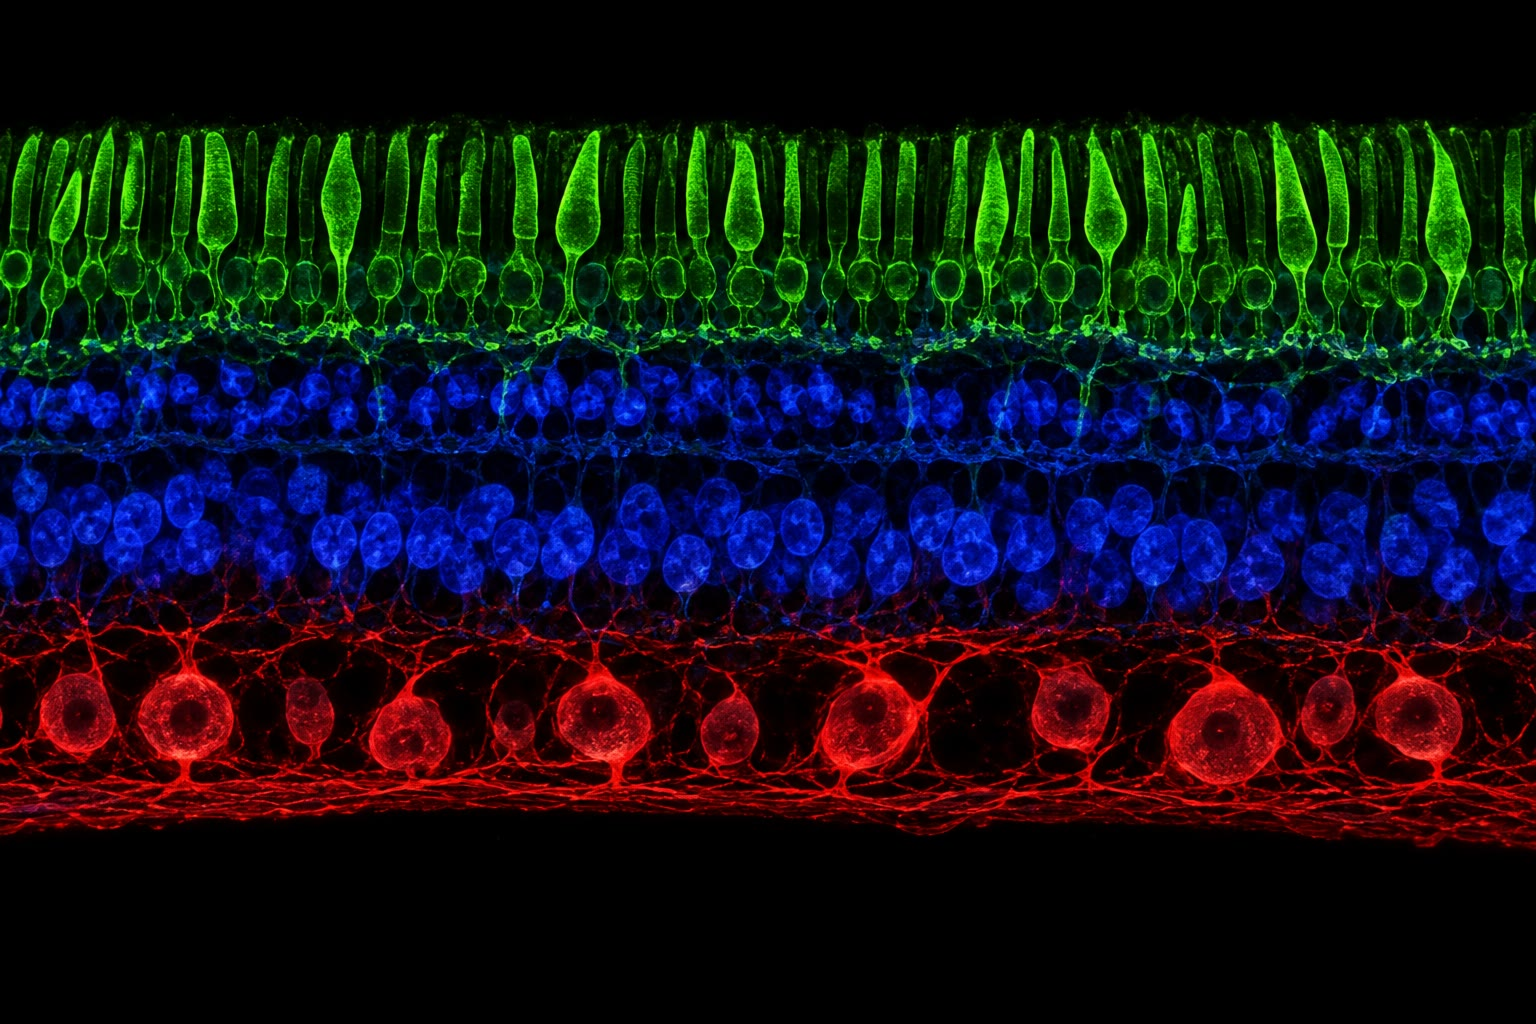
\includegraphics[width=0.46\linewidth]{images/book5/ai/b5-18-retina-section.jpg}\hspace{0.04\linewidth}
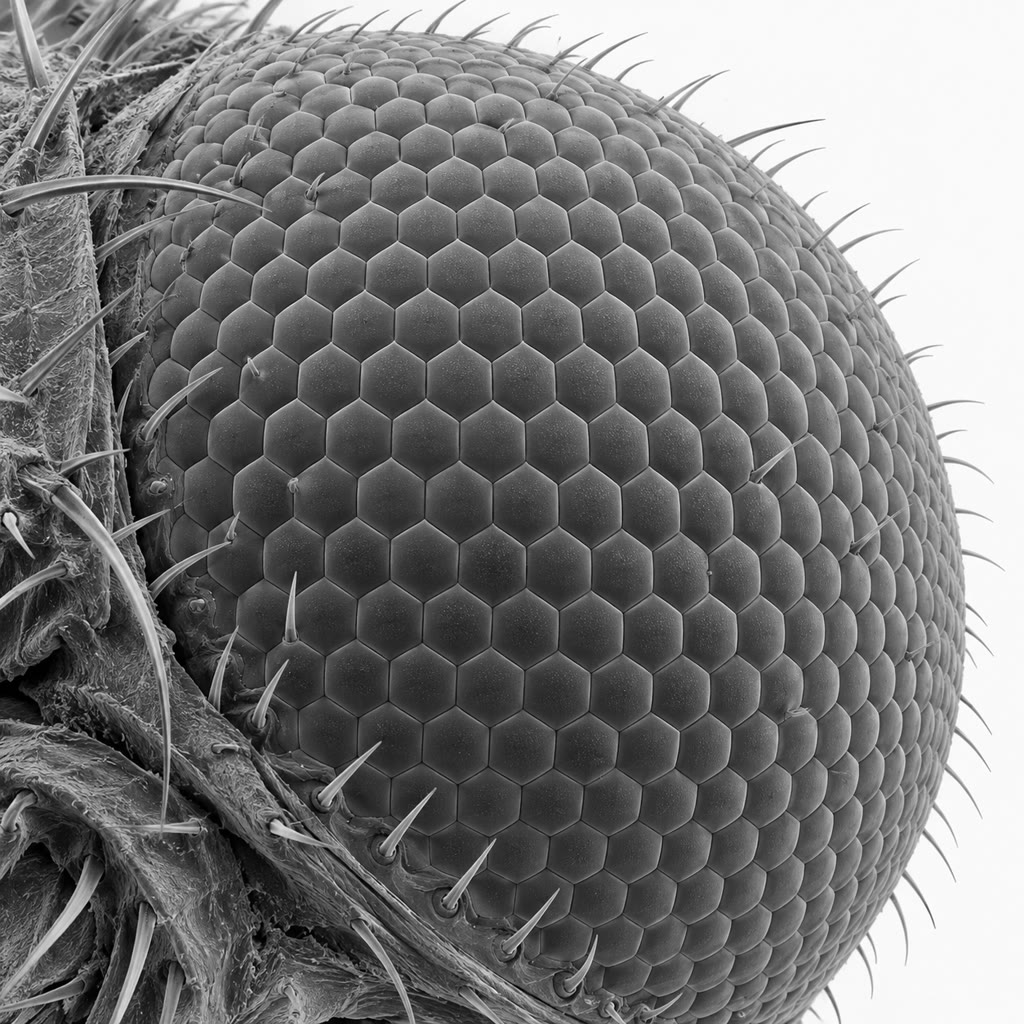
\includegraphics[width=0.36\linewidth]{images/book5/ai/b5-18-compound-eye.jpg}

{\small Kiri: sebuah irisan \omterm{def:b3:sensory-systems:retina}{retina}, dengan fotoreseptornya (hijau) di
belakang, lalu sel bipolar dan horizontalnya, lalu \omterm{def:b3:sensory-systems:retina}{sel ganglionnya}
(merah) yang aksonnya berangkat ke otaknya. Kanan: mata majemuk seekor
lalat, ratusan lensa terpisah yang masing-masing berreseptor sendiri --- sebuah
penyelesaian yang berbeda bagi masalah yang sama.}
\end{omfigure}

\section{Pendengaran dan keseimbangan}

\begin{definition}[Koklea]\label{def:b3:sensory-systems:cochlea}
\index{koklea}\index{membran basilar}\index{tonotopi}\index{sel rambut}%
\index{stereosilium}\index{kaitan ujung}\index{desibel}
Bunyi adalah sebuah gelombang tekanan; masalah telinganya adalah mendeteksi
perubahan tekanan sebesar beberapa puluh mikropascal di udara lalu menyortirnya
menurut frekuensi. Gendang telinganya dan ketiga tulang telinga tengahnya
memusatkan gaya dari \qty{55}{mm^2} gendangnya ke \qty{3}{mm^2} tingkap
lonjongnya, yang menaikkan tekanannya sekitar dua puluh kali lipat --- yakni
pemadanan impedans antara udara dan cairan telinga dalamnya, yang tanpanya
kebanyakan bunyinya akan terpantul. Di dalam \emph{koklea}, sebuah tabung terpilin
sepanjang \qty{35}{mm}, gelombang tekanannya mengembara sepanjang \emph{membran
basilar}, yang sempit dan kaku pada pangkalnya dan lebar dan lemas pada
puncaknya; tiap frekuensi membuat membrannya bergetar paling kuat pada satu tempat
--- frekuensi tinggi dekat pangkalnya, rendah dekat puncaknya --- yakni sebuah
peta \emph{tonotopis} yang dibaca otaknya sebagai tinggi nada. Pada membrannya duduk
\emph{sel rambut}: \num{3500} sel rambut dalam dalam sebuah baris tunggal,
yang masing-masing bermahkota seberkas \emph{stereosilium} yang disambung ujung ke ujung oleh
\emph{kaitan ujung} yang halus; membengkokkan berkasnya ke arah \omterm{def:b3:cytoskeleton-motility:cilia}{silium} tertingginya
meregangkan kaitannya lalu menarik terbuka saluran kation dalam hitungan mikrodetik,
tanpa pesuruh kedua mana pun, dan kalium mengalir masuk dari
endolimfanya, yang susunannya tak lazim dan potensialnya $+\qty{80}{mV}$ memberi
sebuah gaya penggerak \qty{150}{mV}. Sel rambut dalamnya mengisyarati
saraf pendengarannya; \num{12000} sel rambut luarnya, yang digerakkan gerak yang sama,
mengerut dan memanjang bersama bunyinya lewat protein motor
prestin lalu memompakan tenaga kembali ke getaran membrannya --- yakni sebuah
pelipat ganda yang menajamkan penalaannya seratus kali lipat dan yang gagal pada kebanyakan
ketulian. Keamatannya diukur dalam \emph{desibel}: $L = 10\log_{10}
(I/I_{0})$, dengan $I_{0} = \qty{1e-12}{W/m^2}$ ambang pendengarannya;
telinganya bekerja sepanjang \qty{120}{dB}, yakni sejuta juta kali lipat dalam keamatan.
\end{definition}

\begin{omfigure}
\begin{tikzpicture}[every node/.style={font=\scriptsize}, >=stealth]
  % unrolled cochlea
  \begin{scope}
    \draw[thick, omDef, fill=omDef!10] (0,0.9) -- (7,1.4) -- (7,-1.4) -- (0,-0.9) -- cycle;
    \draw[very thick, omProp] (0,0.15) -- (7,-0.15); \draw[very thick, omProp] (0,-0.15) -- (7,0.15);
    \node[above] at (0.8,1.05) {pangkal: sempit, kaku}; \node[above] at (6.2,1.5) {puncak: lebar, lemas};
    \node[left, align=right] at (-0.1,0) {tingkap lonjong\\(sanggurdi)};
    \foreach \x/\f in {0.9/\qty{16}{kHz}, 2.3/\qty{4}{kHz}, 3.8/\qty{1}{kHz}, 5.4/\qty{250}{Hz}, 6.6/\qty{60}{Hz}} { \draw[omThm, thick] (\x,-0.55) -- (\x,0.55); \node[below, omThm] at (\x,-0.65) {\f}; }
    \node[below, align=center] at (3.5,-1.7) {membran basilar (oranye): tiap frekuensi\\bergetar paling kuat pada satu tempat --- tonotopi};
  \end{scope}
  % hair cell mechanism
  \begin{scope}[xshift=7.5cm, yshift=-0.6cm]
    \draw[thick, fill=omMeth!20] (0,0) rectangle (1.6,1.2); \node[below] at (0.8,-0.05) {sel rambut};
    \foreach \x/\h in {0.35/0.6, 0.65/0.85, 0.95/1.1, 1.25/1.35} \draw[very thick, omMeth!70!black] (\x,1.2) -- (\x,1.2+\h);
    \foreach \x/\h/\xx/\hh in {0.35/0.6/0.65/0.85, 0.65/0.85/0.95/1.1, 0.95/1.1/1.25/1.35} \draw[omThm, thick] (\x,1.2+\h) -- (\xx,1.2+\hh-0.1);
    \draw[->, thick] (1.9,2.3) -- (2.4,2.3) node[right, align=left, font=\tiny] {bengkokkan ke yang tertinggi:\\kaitan ujungnya meregang,\\salurannya terbuka dalam\\$\unit{\micro s}$; K$^{+}$ masuk\\(dorongan \qty{150}{mV})};
    \node[above, align=center] at (0.8,2.7) {stereosilium yang disambung\\kaitan ujung (merah)};
  \end{scope}
\end{tikzpicture}

{\small Kiri: \omterm{def:b3:sensory-systems:cochlea}{koklea} yang dibuka gulungannya --- \omterm{def:b3:sensory-systems:cochlea}{membran basilarnya} berjenjang dari
kaku ke lemas, dan tiap frekuensi memuncak pada tempatnya sendiri. Kanan: sebuah
berkas rambut, yang \omterm{def:b3:sensory-systems:cochlea}{kaitan ujungnya} membuka saluran transduksinya
secara mekanis ketika berkasnya dibengkokkan.}
\end{omfigure}

\begin{proof}[Bukti eksperimental]
Von Békésy (dasawarsa 1940-an) membuka \omterm{def:b3:sensory-systems:cochlea}{koklea} mayat, menaburkan
butir perak pada \omterm{def:b3:sensory-systems:cochlea}{membran basilarnya} lalu menyaksikan di bawah
cahaya stroboskopis ketika nada murni menegakkan sebuah gelombang mengembara yang puncaknya
terletak makin dekat ke pangkalnya makin tinggi nadanya --- yakni sandi tempat, yang karenanya
ia menerima hadiah Nobel pada tahun 1961. Hudspeth (dasawarsa 1980-an) mendorong sebuah
berkas rambut tunggal dengan sebuah serat kaca lalu merekam arusnya: arusnya mengalir
dalam \qty{10}{\micro s} sesudah dorongannya, jauh terlalu cepat bagi runtunan enzim mana pun,
sebanding dengan seberapa jauh berkasnya bergerak ke arah baris tertingginya,
dan arusnya lenyap ketika \omterm{def:b3:sensory-systems:cochlea}{kaitan ujungnya} dipotong dengan sebuah pengelat
kalsium. Pergerbangannya bersifat mekanis --- kaitannya menarik salurannya terbuka ---
dan itulah sebabnya pendengaran adalah indra yang tercepat dan sebabnya
transdusernya dimusnahkan bunyi keras yang memutuskan kaitannya.
\end{proof}

\begin{example}[Angka telinganya]\label{ex:b3:sensory-systems:ear-numbers}
Pada ambang pendengarannya, \omterm{def:b3:sensory-systems:cochlea}{membran basilarnya} bergerak sekitar
\qty{0.1}{nm} dan amplitudo tekanannya \qty{20}{\micro Pa}, yakni
dua per miliar tekanan atmosfer; pada \qty{120}{dB} tekanannya
sejuta kali lebih besar dan gerak membrannya berpuluh nanometer. Sebuah
telinga muda mendengar dari \qty{20}{Hz} sampai \qty{20}{kHz} lalu memisahkan nada
yang berjarak \qty{0.3}{\%}, dengan pembedaan sandi tempatnya ditajamkan
\omterm{def:b3:sensory-systems:cochlea}{sel rambut} luarnya. Ke-\num{30000} serat saraf pendengarannya menyala selangkah
dengan gelombang tekanannya sampai sekitar \qty{4}{kHz} (penguncian fase),
yang mengusung ketepatan waktu sampai kecermatan puluhan mikrodetik, yang darinya
otaknya menghitung arah sebuah bunyi dari selisih kedatangannya pada
kedua telinganya --- sekecil \qty{10}{\micro s}. Organ keseimbangannya memakai
\omterm{def:b3:sensory-systems:cochlea}{sel rambut} yang sama: di dalam \emph{saluran setengah lingkaran}, kelembaman
cairannya membengkokkannya ketika kepalanya berputar (percepatan sudut), dan di dalam
organ otolitnya selapis hablur kalsium karbonat membebaninya
dengan gravitasi dan percepatan lurus.
\end{example}

\begin{omfigure}
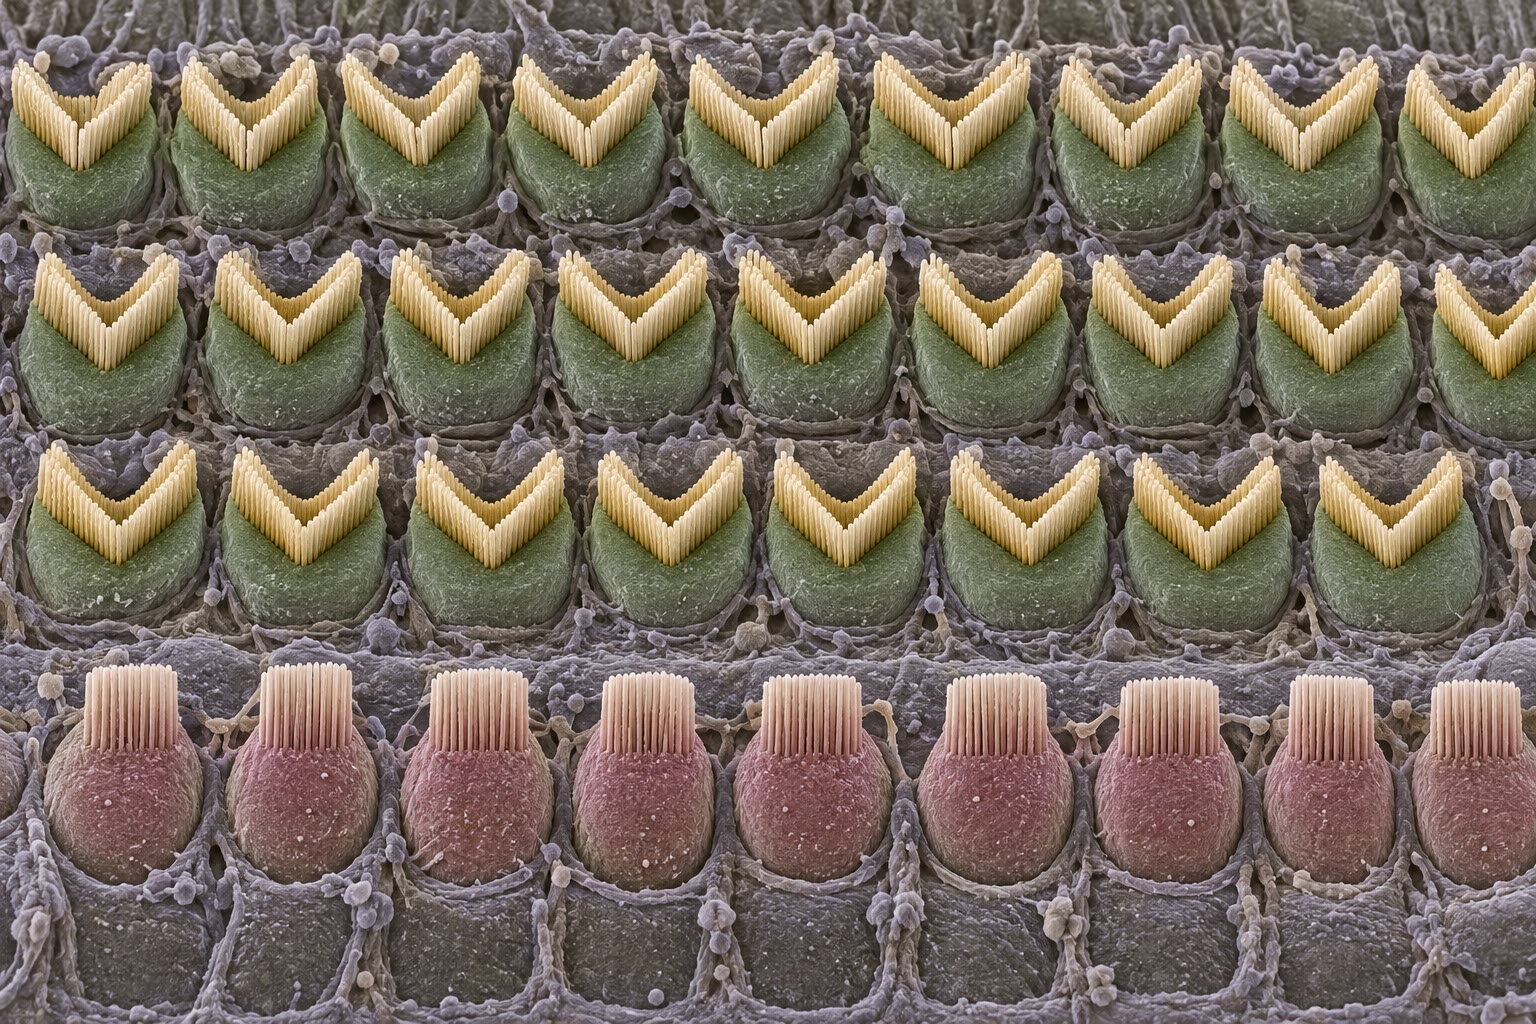
\includegraphics[width=0.54\linewidth]{images/book5/ai/b5-18-cochlea-hair-cells.jpg}

{\small Organ Corti dari atas: tiga baris \omterm{def:b3:sensory-systems:cochlea}{sel rambut} luar
dengan berkas berbentuk V, satu baris \omterm{def:b3:sensory-systems:cochlea}{sel rambut} dalam. \omterm{def:b3:sensory-systems:cochlea}{Kaitan ujung} tiap berkas
membuka salurannya; sel luarnya melipatgandakan, sel dalamnya
melaporkan.}
\end{omfigure}

\section{Indra kimia}

\begin{definition}[Penciuman dan pengecapan]\label{def:b3:sensory-systems:chemical}
\index{reseptor penciuman}\index{sandi kombinatoris}\index{glomerulus}\index{pengecapan}
Penciuman bermula di sepetak epitelium di puncak hidung, tempat
sekitar sepuluh juta \emph{neuron indra penciuman} masing-masing mengungkapkan satu
gen \emph{reseptor penciuman} dari sekitar $400$ pada manusia (\num{1100}
pada mencit, keluarga gen terbesar pada kedua genom) --- yakni reseptor
tergandeng-protein~G yang mengikat molekul zat bau di dalam sebuah kantung lalu, lewat
AMP siklik, membuka sebuah saluran. Tiap reseptor mengikat beberapa zat bau dan
tiap zat bau mengikat beberapa reseptor, sehingga sebuah bau adalah sebuah
\emph{sandi kombinatoris}, yakni sebuah pola keaktifan di seluruh $400$
jenis reseptornya, dan sebuah perubahan satu karbon pada sebuah molekul mengubah
polanya dan baunya. Semua neuron yang mengungkapkan satu reseptor mengirim
aksonnya ke satu atau dua \emph{glomerulus} yang sama di dalam bulbus penciumannya,
sehingga bulbusnya memuat sebuah peta yang di dalamnya tiap bau adalah sebuah pola
ruang glomerulus yang aktif, yang dibaca korteksnya tanpa melewati
\omterm{def:b3:nervous-systems:plan}{talamus}. Pengecapan lebih sederhana: lima modalitas, masing-masing sebuah
\omterm{def:b3:sensory-systems:principles}{jalur berlabel} dari sel reseptornya sendiri --- manis, gurih, dan pahit
lewat reseptor tergandeng-protein~G (satu reseptor manis, satu gurih,
sekitar dua puluh lima pahit), asin lewat sebuah saluran natrium, asam lewat
sebuah saluran proton --- dan sisa dari apa yang kita sebut cita rasa adalah baunya,
yang mencapai hidungnya lewat belakang mulutnya.
\end{definition}

\begin{proof}[Bukti eksperimental]
Buck dan Axel (1991) menalar bahwa reseptor zat bau tentulah berupa
reseptor tergandeng-protein~G yang diungkapkan hanya di dalam epitelium penciumannya,
lalu menemukan dengan PCR memakai pemula merosot sebuah keluarga berisi ratusan
gen semacam itu, yang diungkapkan di sana dan tidak di tempat lain --- yakni reseptor bagi
penciuman, yang tak dikenal selama seabad. Hibridisasi di tempat menunjukkan satu reseptor
tiap neuron dan \omterm{def:b3:nervous-systems:circuits}{pemusatan} neuron sejenis pada \omterm{def:b3:sensory-systems:chemical}{glomerulus} tunggal;
Malnic, Buck, dan rekannya (1999) merekam neuron tunggal lalu menunjukkan
bahwa tiap zat bau mengaktifkan beberapa jenis reseptor dan tiap reseptor
beberapa zat bau --- itulah \omterm{def:b3:sensory-systems:chemical}{sandi kombinatorisnya}. Bushdid dan rekannya
(2014) meminta subjek membedakan campuran lalu menaksir bahwa
manusia dapat membedakan lebih daripada sejuta juta bau, jauh melampaui
beberapa ribu yang lazim dipercaya.
\end{proof}

\begin{proposition}[Kapasitas sebuah sandi kombinatoris]\label{prop:b3:sensory-systems:combinatorial}
\index{sandi kombinatoris!kapasitas}
Dengan $R$ jenis reseptor yang masing-masing entah aktif atau bungkam, sebuah bau dapat
diwakili oleh sembarang dari $2^{R}$ pola; dengan $R = 400$ itu adalah
$10^{120}$, dan bahkan bila hanya pola dengan tepat $10$ jenis yang aktif
ditinjau, terdapat $\binom{400}{10} \approx 3\times 10^{20}$.
Pembedaannya dibatasi bukan oleh sandinya melainkan oleh derau
reseptornya dan oleh pembacaan otaknya: sebuah sandi \omterm{def:b3:sensory-systems:principles}{jalur berlabel} dengan satu
reseptor tiap bau akan mengizinkan $400$ bau, sedangkan \omterm{def:b3:sensory-systems:chemical}{sandi kombinatoris}
mengizinkan lebih banyak daripada molekul yang ada untuk dibaui. Ongkosnya adalah bahwa sebuah
reseptor tunggal mengatakan sedikit saja kepada otaknya dengan sendirinya; polanya harus
dibaca sebagai sebuah keseluruhan, dan itulah yang dikerjakan peta \omterm{def:b3:sensory-systems:chemical}{glomerulus} dan korteks
penciumannya.
\end{proposition}

\begin{omfigure}
\begin{tikzpicture}[every node/.style={font=\scriptsize}, >=stealth]
  % receptor rows, odorant columns
  \foreach \i/\lab in {1/reseptor A, 2/reseptor B, 3/reseptor C, 4/reseptor D, 5/reseptor E} \node[left] at (-0.1,-0.7*\i) {\lab};
  \foreach \j/\lab in {1/heksanol, 2/heptanol, 3/oktanol, 4/limonena} \node[above, rotate=0] at (1.2*\j-0.6,-0.35) {\lab};
  \foreach \i/\j/\v in {1/1/100, 1/2/30, 2/1/60, 2/2/100, 2/3/50, 3/2/40, 3/3/100, 3/4/20, 4/3/70, 5/4/100, 1/4/30} \fill[omThm!\v] (1.2*\j-1.15,-0.7*\i-0.3) rectangle (1.2*\j-0.05,-0.7*\i+0.3);
  \foreach \i in {1,...,5} \foreach \j in {1,...,4} \draw[gray!50] (1.2*\j-1.15,-0.7*\i-0.3) rectangle (1.2*\j-0.05,-0.7*\i+0.3);
  \node[below, align=center] at (2.1,-4.1) {tiap zat bau mengaktifkan sehimpunan reseptor,\\tiap reseptor sehimpunan zat bau:\\baunya adalah kolomnya};
  % glomerular map
  \begin{scope}[xshift=9.2cm, yshift=-2.2cm]
    \draw[thick, omDef!60, fill=omDef!8] (0,0) ellipse (2.6 and 1.7); \node[above] at (0,1.75) {bulbus penciuman: glomerulus};
    \foreach \p in {(-1.8,0.6),(-1.0,1.0),(-0.2,0.7),(0.8,1.0),(1.7,0.5),(-1.6,-0.4),(-0.6,-0.6),(0.4,-0.3),(1.3,-0.7),(0.1,0.2)} \draw[omDef!70, fill=omDef!25] \p circle (0.25);
    \fill[omThm!80] (-1.0,1.0) circle (0.25); \fill[omThm!50] (0.4,-0.3) circle (0.25); \fill[omThm!80] (1.7,0.5) circle (0.25);
    \node[below, align=center] at (0,-1.8) {semua neuron dari satu jenis reseptor\\memusat pada satu glomerulus: sebuah bau adalah\\sebuah pola ruang (merah) yang dibaca korteksnya};
  \end{scope}
\end{tikzpicture}

{\small \omterm{def:b3:sensory-systems:chemical}{Sandi kombinatoris} penciuman. Kiri: sebuah matriks
reseptor-lawan-zat-bau, yang di dalamnya tiap bau adalah sebuah pola menurun sebuah kolom. Kanan:
polanya yang dibentangkan pada \omterm{def:b3:sensory-systems:chemical}{glomerulus} bulbusnya.}
\end{omfigure}

\begin{omfigure}
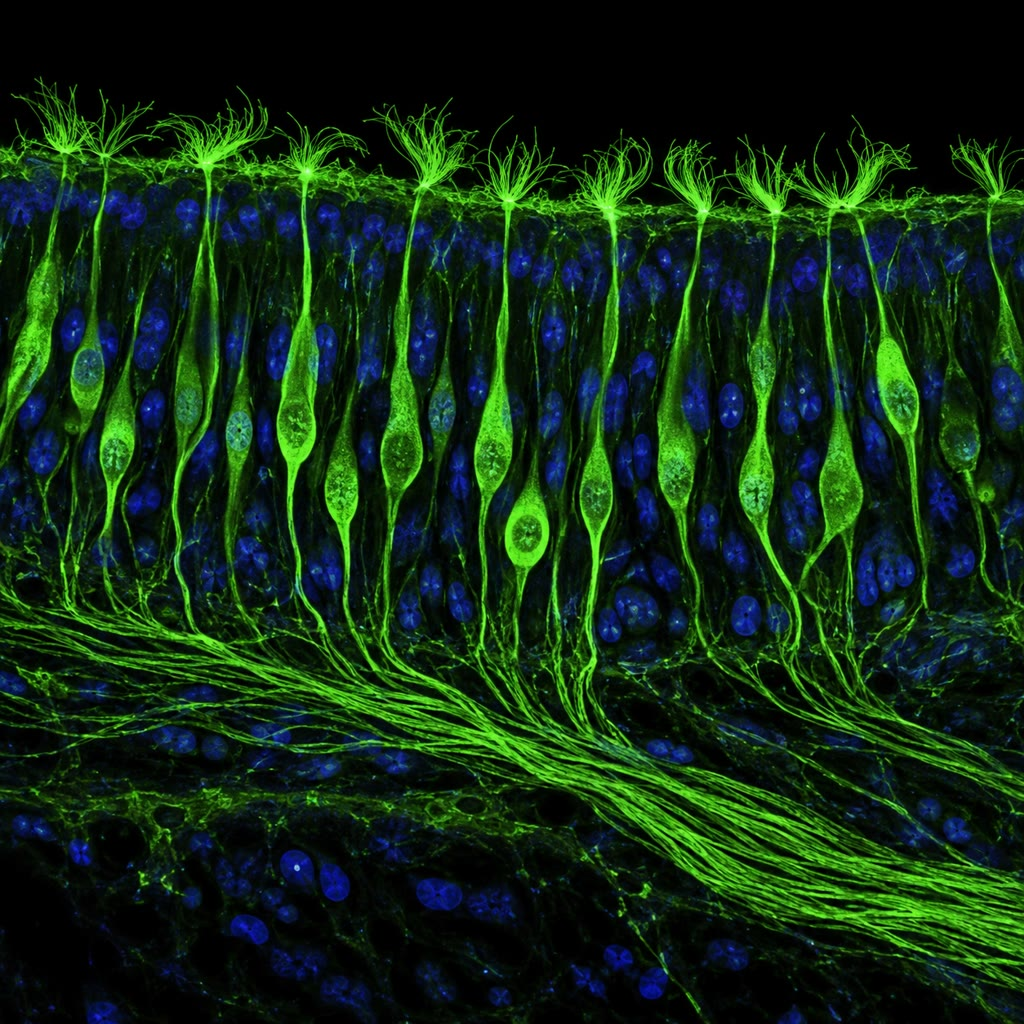
\includegraphics[width=0.40\linewidth]{images/book5/ai/b5-18-olfactory-epithelium.jpg}

{\small Epitelium penciuman: neuron indra (hijau) dengan
dendrit bersilium di permukaannya, tempat zat baunya mengikat, dan akson yang
berkas-berkas di bawahnya menuju bulbusnya. Tiap neuron mengungkapkan satu gen reseptor dari
keempat ratusnya.}
\end{omfigure}

\section{Sentuhan, suhu, nyeri, dan indra yang tidak kita punyai}

\begin{definition}[Penginderaan somatik]\label{def:b3:sensory-systems:somato}
\index{mekanoreseptor}\index{saluran Piezo}\index{saluran TRP}%
\index{nosiseptor}\index{propriosepsi}
Kulitnya memuat beberapa jenis \emph{mekanoreseptor}, masing-masing sebuah akson
yang berakhir di dalam kapsulnya sendiri: sel Merkel bagi tekanan halus dan tekstur
(beradaptasi lambat, bermedan kecil), badan Meissner bagi sentuhan ringan
dan selip (beradaptasi cepat), badan Pacini yang dalam di kulit bagi
getaran (beradaptasi sangat cepat, bermedan raksasa), ujung Ruffini bagi
regangan. Transduser pada kebanyakannya adalah \emph{Piezo2}, yakni sebuah saluran
ion raksasa dengan sebuah baling-baling bersudu yang terbuka ketika selaputnya
teregang; tanpanya sentuhan dan indra kedudukan tubuhnya
hilang, dan saluran yang sama di paru dan kandung kemih mengindera
pengisiannya. \emph{Suhu} diindera saluran keluarga TRP yang
ditala pada jangkauan yang berbeda --- TRPV1, yang dibuka panas di atas
\qty{43}{\celsius} dan oleh kapsaisin, dan itulah sebabnya cabai terasa ``panas'';
TRPM8, yang dibuka dingin dan oleh mentol --- dan \emph{nyeri} oleh ujung saraf
bebas, yakni \emph{nosiseptor}, yang menanggapi panas, tekanan, atau bahan kimia
yang merusak (proton, ATP, bradikinin) dan yang ambangnya
diturunkan \omterm{def:b3:innate-immunity:inflammation}{peradangan} (\cref{ch:b3:innate-immunity}).
\emph{Propriosepsi}, yakni indra tempat anggota badannya berada, datang dari
kumparan otot dan organ tendon \cref{ch:b3:nervous-systems}
dan dari Piezo2 di dalam kapsul sendinya. Kerapatan reseptornya menetapkan
ketajamannya: dua titik yang berjarak \qty{2}{mm} dibedakan pada sebuah ujung jari,
berjarak \qty{40}{mm} pada punggungnya.
\end{definition}

\begin{method}[Mengukur sebuah indra]\label{met:b3:sensory-systems:psychophysics}
\index{psikofisika}\index{ambang}\index{pembedaan dua titik}
Untuk mencirikan sebuah saluran indra: (1) temukanlah \emph{ambang
mutlaknya} dengan menyajikan rangsang berkeamatan berjenjang berkali-kali lalu
mencocokkan bagian yang terdeteksi --- yakni keamatan yang terdeteksi separuh waktunya
--- sebagaimana dilakukan Hecht; (2) temukanlah \emph{ambang bedanya} pada beberapa
keamatan lalu periksalah \omterm{thm:b3:sensory-systems:weber}{hukum Weber}; (3) petakanlah \emph{ketajaman ruangnya} dengan
dua rangsang pada pemisahan yang beragam (uji dua titik pada kulit, sebuah
kisi pada \omterm{def:b3:sensory-systems:retina}{retina}); (4) petakanlah \emph{ketajaman waktunya} dengan kerlipan
atau ketikan (sebuah kerlipan melebur pada sekitar \qty{60}{Hz} pada penglihatan siang);
(5) pada seekor hewan, rekamlah dari serat aferen tunggal sambil mengenakan
rangsang yang sama lalu padankanlah ambang sarafnya dengan ambang tingkah lakunya
--- psikofisika dan fisiologinya mestinya sepakat, dan di tempat keduanya
tidak sepakat, selisihnya adalah apa yang ditambahkan otaknya.
\end{method}

\begin{remark}[Hewan lain, indra lain]\label{rem:b3:sensory-systems:others}
Tiap indra di sini punya sebuah versi yang didorong lebih jauh oleh seekor hewan, dan ada
indra yang tidak kita punyai. Hiu dan pari mengindera medan mikrovolt
detak jantung mangsanya lewat saluran berisi jeli; ikan listrik membaca
perubahan medannya sendiri untuk melihat di dalam gelap. Ular berbisa mencitrakan
mangsa yang hangat dengan lubang yang peka inframerah; kelelawar dan lumba-lumba berekolokasi,
dengan menakar waktu gema panggilannya sendiri sampai beberapa mikrodetik lalu mengemudikan
frekuensi panggilannya untuk menjejaki seekor ngengat; lebah melihat ultraungu dan
pengutuban cahaya langit lalu bernavigasi dengannya; burung yang bermigrasi dan
penyu mengindera medan magnet Bumi lewat sebuah mekanisme yang masih
diperdebatkan. Hidung seekor anjing punya empat puluh kali neuron reseptor kita dan sepertiga
otaknya untuk membacanya; seekor burung hantu mendengar seekor tikus di bawah salju.
Asasnya tidak berubah --- sebuah transduser, sebuah \omterm{def:b3:sensory-systems:principles}{jalur berlabel}, sebuah sandi,
pemampatan, sebuah peta --- dan keragamannya adalah apa yang telah dilakukan evolusi
dengannya.
\end{remark}

\section{Latihan}

\begin{exercise}[$\star$]\label{exo:b3:sensory-systems:1}
Jelaskanlah bagaimana otaknya tahu apakah sebuah deretan lecutan datang dari
matanya atau telinganya, mengingat lecutannya serupa.
\end{exercise}

\begin{exercise}[$\star$]\label{exo:b3:sensory-systems:2}
Mengapa cahaya menghiperpolarisasi sebuah fotoreseptor, dan apa itu arus
gelap?
\end{exercise}

\begin{exercise}[$\star$]\label{exo:b3:sensory-systems:3}
Sebuah bisikan \qty{20}{dB}, sebuah percakapan \qty{60}{dB}, sebuah konser rok
\qty{110}{dB}. Hitunglah keamatan masing-masing dalam W/m$^{2}$ dan
nisbah antara yang ternyaring dan yang terlembut.
\end{exercise}

\begin{exercise}[$\star$]\label{exo:b3:sensory-systems:4}
Nyatakanlah kelima modalitas \omterm{def:b3:sensory-systems:chemical}{pengecapan} dan jenis reseptornya, lalu jelaskanlah
mengapa sebuah pilek menghalangi ``rasa'' makanan.
\end{exercise}

\begin{exercise}[$\star\star$]\label{exo:b3:sensory-systems:5}
Pecahan Weber bagi bobot adalah $0.02$. Mulai dari sebuah bobot
\qty{100}{g}, berapa langkah yang baru terasa terletak di antaranya dan
\qty{10}{kg}? Pakailah rumus Fechner lalu periksalah dengan mencacah langkah
berfaktor $1.02$.
\end{exercise}

\begin{exercise}[$\star\star$]\label{exo:b3:sensory-systems:6}
Dengan memakai \cref{thm:b3:sensory-systems:hecht}, hitunglah $P_{\text{lihat}}$ bagi
$a = 2$, $6$, dan $12$ foton terserap dengan ambang $n = 6$.
Pada $a$ berapa kilatannya terlihat separuh waktunya? Bila \qty{10}{\%} foton
pada korneanya terserap, berapa banyak yang harus dihantarkan kilatannya?
\end{exercise}

\begin{exercise}[$\star\star$]\label{exo:b3:sensory-systems:7}
Telinga tengahnya memusatkan gaya dari \qty{55}{mm^2} ke
\qty{3}{mm^2} dengan sebuah tuas $1.3$. Dengan faktor berapa tekanannya
naik, dan dalam \omterm{def:b3:sensory-systems:cochlea}{desibel}? Mengapa telinga seseorang dengan tulang
telinga tengah yang berlekatan (otosklerosis) lebih tumpul berpuluh \omterm{def:b3:sensory-systems:cochlea}{desibel}?
\end{exercise}

\begin{exercise}[$\star\star$]\label{exo:b3:sensory-systems:8}
Jelaskanlah mengapa arus transduksi sebuah \omterm{def:b3:sensory-systems:cochlea}{sel rambut} muncul dalam
hitungan mikrodetik sedangkan arus sebuah fotoreseptor memakan puluhan
milidetik, dan apa yang diperoleh tiap indra dari rancangannya.
\end{exercise}

\begin{exercise}[$\star\star$]\label{exo:b3:sensory-systems:9}
Seekor mencit punya \num{1100} jenis reseptor dan seorang manusia $400$. Bila sebuah bau
mengaktifkan sekitar \qty{5}{\%} jenisnya, berapa banyak pola yang tepat
sebesar itu yang tersedia bagi masing-masing (pakailah $\binom{R}{k}$ dengan $k = 0.05R$,
dan hampiran Stirling $\ln\binom{R}{k} \approx R\,H(k/R)$ dengan
$H(p) = -p\ln p - (1-p)\ln(1-p)$)?
\end{exercise}

\begin{exercise}[$\star\star\star$]\label{exo:b3:sensory-systems:10}
Sebuah \omterm{def:b3:sensory-systems:retina}{sel batang} mengisomerkan sebuah \omterm{def:b3:sensory-systems:retina}{rodopsin} secara spontan sekali tiap \qty{40}{s} di
dalam gelap. Pada sepetak $500$ \omterm{def:b3:sensory-systems:retina}{sel batang} yang diamati selama sebuah jendela \qty{0.1}{s},
berapa cacah rata-rata peristiwa spontannya, dan berapa peluang
bahwa enam atau lebih terjadi secara kebetulan? Jelaskanlah mengapa otaknya menetapkan
ambangnya pada sekitar enam dan bukan pada satu.
\end{exercise}

\begin{exercise}[$\star\star\star$]\label{exo:b3:sensory-systems:11}
Saraf pendengarannya mengunci lecutannya pada fase bunyinya sampai
\qty{4}{kHz}, dengan gugupan sekitar \qty{20}{\micro s}. Bunyi mengembara
pada \qty{340}{m/s} dan telinganya berjarak \qty{20}{cm}. Berapa
penundaan antartelinga yang terbesar, daya pisah sudut berapa yang diberikan sebuah
pembedaan \qty{10}{\micro s} dekat garis tengahnya, dan mengapa
sandi tempat, bukan ketepatan waktu, yang melayani di atas \qty{4}{kHz}?
\end{exercise}

\begin{exercise}[$\star\star\star$]\label{exo:b3:sensory-systems:12}
\omterm{def:b3:sensory-systems:principles}{Penghambatan lateral} membuat sebuah medan kelabu seragam di sebelah medan gelap tampak
lebih terang di perbatasannya. Modelkanlah sebaris reseptor yang masing-masing dipacu cahayanya
sendiri $I_{i}$ dan dihambat oleh sebuah pecahan $w$ cahaya tiap tetangganya,
$r_{i} = I_{i} - w(I_{i-1} + I_{i+1})$, lalu hitunglah tanggapannya melintasi
sebuah tangga dari $I = 1$ ke $I = 2$ dengan $w = 0.2$. Apa yang diperoleh \omterm{def:b3:sensory-systems:retina}{retinanya}
dan apa yang hilang darinya karena hal ini?
\end{exercise}

\section{Soal: Sebatang Lilin yang Dilihat dari Jauh}

\begin{problem}[{Soal akhir pekan --- foton sebatang lilin yang dicacah ke dalam
sebuah mata yang jauh, pendeteksian kilatannya yang dihitung dari statistika Poisson
dan pelipat ganda sel batangnya, desibel sebuah konser yang diubah menjadi gerak gendang telinga
dan arus sel rambut, serta sandi sebuah hidung yang dicacah, berakhir pada
jarak yang padanya lilinnya terlihat, tekanan pada gendang telinganya,
dan pola yang dapat dibentuk sebuah hidung}]
\label{pb:b3:sensory-systems:1}
Data: sebatang lilin memancarkan sekitar \qty{0.01}{W} cahaya tampak, pada
\qty{550}{nm} (tenaga foton $3.6\times 10^{-19}$ J). Sebuah manik mata yang
teradaptasi gelap selebar \qty{7}{mm}; \qty{10}{\%} foton yang memasuki matanya
diserap \omterm{def:b3:sensory-systems:retina}{rodopsin}; matanya mengintegralkan sepanjang \qty{0.1}{s};
ambangnya $6$ foton terserap. Tiap foton terserap menutup $200$
saluran lalu memangkas arus gelapnya sebesar \qty{1}{pA} selama \qty{0.2}{s};
arus gelap sebuah \omterm{def:b3:sensory-systems:retina}{sel batang} \qty{30}{pA}. Bunyi: $I_{0} =
\qty{1e-12}{W/m^2}$; gendang telinganya berluas \qty{55}{mm^2}; sebuah berkas rambut
setinggi \qty{5}{\micro m} pada ambangnya melentur sebesar \qty{0.3}{nm}.
Penciuman: $R = 400$ reseptor; arus transduksi sebuah \omterm{def:b3:sensory-systems:cochlea}{sel rambut} adalah
\qty{100}{pA} pada kejenuhannya.

\medskip
\noindent\textbf{Bagian I --- Foton.}
\begin{enumerate}
  \item Berapa banyak foton tiap detik yang dipancarkan lilinnya?
  \item Pada jarak $d$ fotonnya tersebar pada sebuah bola berluas
        $4\pi d^{2}$. Berapa banyak yang memasuki manik matanya tiap detik pada
        \qty{1}{km}? Pada \qty{10}{km}?
  \item Berapa banyak yang terserap dalam satu jendela integrasi pada tiap
        jaraknya? Apakah lilinnya terlihat (ambang $6$)?
  \item Temukanlah jarak yang padanya cacah rata-rata yang terserap dalam sebuah jendela
        sama dengan $6$. Dengan statistika Poisson, berapa bagian jendela yang
        melampaui ambangnya di sana?
  \item Pada jarak pertanyaan 4, berapa peluang bahwa sebuah
        jendela \qty{0.1}{s} tertentu tidak memuat satu foton pun? Mengapa sebuah
        bintang samar tampak berkerlip?
  \item Di bawah bulan purnama, \omterm{def:b3:sensory-systems:retina}{sel batang} yang sama menyerap $10^{4}$ foton tiap
        jendela dari langitnya. Jelaskanlah mengapa lilin pada \qty{10}{km} itu
        lalu tak terlihat walaupun ia menghantarkan foton yang sama.
\end{enumerate}

\medskip
\noindent\textbf{Bagian II --- Pelipat ganda \omterm{def:b3:sensory-systems:retina}{sel batangnya}.}
\begin{enumerate}[resume]
  \item Satu foton menutup $200$ saluran lalu memangkas arusnya sebesar
        \qty{1}{pA}. Arus berapa yang diusung satu saluran, dan berapa banyak
        kation tiap detik itu ($e = \qty{1.6e-19}{C}$)?
  \item Berapa bagian arus gelapnya yang disingkirkan satu foton? Berapa
        banyak foton serentak yang akan mematikan \omterm{def:b3:sensory-systems:retina}{sel batangnya} sama sekali
        (kejenuhan)?
  \item Tanggapannya bertahan \qty{0.2}{s}. Berapa banyak kation yang dicegah
        satu foton dari masuk? Berapa bati muatan tiap
        fotonnya?
  \item Pada siang hari $10^{5}$ foton tiap detik mencapai sebuah \omterm{def:b3:sensory-systems:retina}{sel batang}. Apa yang terjadi
        padanya, dan mengapa \omterm{def:b3:sensory-systems:retina}{sel kerucut}, yang lebih sedikit beradaptasi dan menjenuh, menjadi
        reseptor siang harinya?
  \item \omterm{def:b3:sensory-systems:retina}{Sel kerucut} memerlukan sekitar $100$ foton untuk mengisyaratkan. Jelaskanlah menurut
        pertukaran antara kepekaan dan kecepatan mengapa \omterm{def:b3:sensory-systems:retina}{sel kerucut} menanggapi dalam
        \qty{20}{ms} dan \omterm{def:b3:sensory-systems:retina}{sel batang} dalam \qty{200}{ms}.
  \item Sebuah \omterm{def:b3:sensory-systems:retina}{rodopsin} mengisomer secara spontan sekali tiap \qty{40}{s}. Pada
        $10^{8}$ \omterm{def:b3:sensory-systems:retina}{sel batang} sebuah mata, berapa banyak foton palsu tiap detik
        yang dihasilkan \omterm{def:b3:sensory-systems:retina}{retinanya}, dan mengapa hal itu tidak membutakan mata yang
        gelap dengan derau? (Pikirkanlah ambangnya dan \omterm{def:b3:sensory-systems:principles}{medan
        reseptifnya}.)
\end{enumerate}

\medskip
\noindent\textbf{Bagian III --- \omterm{def:b3:sensory-systems:cochlea}{Desibel}.}
\begin{enumerate}[resume]
  \item Sebuah konser pada \qty{110}{dB}: keamatan dalam W/m$^{2}$ dan daya
        yang jatuh pada satu gendang telinga.
  \item Berapa banyak tenaga akustik yang diterima gendang telinganya dalam sebuah konser
        dua jam? Bandingkanlah dengan tenaga sebutir hujan yang jatuh
        (\qty{1e-4}{J}).
  \item Ambang pendengarannya pada \qty{0}{dB}: daya pada gendang telinganya
        dan tenaga tiap \qty{10}{ms} --- bandingkanlah dengan tenaga satu
        foton tampak.
  \item Berkas rambutnya melentur \qty{0.3}{nm} pada ambangnya pada sebuah tinggi
        \qty{5}{\micro m}. Sudut berapa itu, dalam derajat? Bandingkanlah
        lenturannya dengan garis tengah sebuah atom hidrogen
        (\qty{0.1}{nm}).
  \item Pemaparan yang lama di atas \qty{85}{dB} merusak \omterm{def:b3:sensory-systems:cochlea}{sel rambut}, dan
        \omterm{def:b3:sensory-systems:cochlea}{sel rambut} tidak pulih pada mamalia. Dua jam pada
        \qty{110}{dB} menghantarkan tenaga sebanyak berapa jam pada
        \qty{85}{dB}?
  \item Jangkauan pendengarannya \qty{120}{dB}. Berapa banyak langkah yang baru
        terasa dalam kenyaringan itu, bila pecahan Weber bagi keamatan adalah
        sekitar $0.25$ (satu \omterm{def:b3:sensory-systems:cochlea}{desibel})?
\end{enumerate}

\medskip
\noindent\textbf{Bagian IV --- Sandi penciuman.}
\begin{enumerate}[resume]
  \item Dengan $400$ reseptor yang masing-masing hidup atau mati, berapa banyak pola? Tulislah
        jawabannya sebagai sebuah pangkat sepuluh.
  \item Bila sebuah bau lazimnya mengaktifkan $20$ reseptor, berapa banyak
        pola semacam itu yang berbeda ($\binom{400}{20}$, pakailah
        Stirling atau logaritma)?
  \item Dua zat bau berbagi $15$ dari $20$ reseptornya. Usulkanlah sebuah
        ukuran jarak keduanya di dalam sandinya lalu jelaskanlah mengapa keduanya
        berbau mirip.
  \item Manusia membedakan sekitar sejuta juta bau. Berapa bagian
        pola pertanyaan 20 yang demikian, dan apa yang membatasi cacahnya
        jauh di bawah kapasitas sandinya?
  \item Seekor mencit dengan \num{1100} reseptor: berapa kali lebih banyak pola
        $20$ daripada manusia, sebagai sebuah pangkat sepuluh?
  \item Sebuah mutasi menghapus satu gen reseptor. Ramalkanlah pengaruhnya pada
        kemampuan membaui pada umumnya dan pada persepsi satu
        zat bau yang mengikat reseptor itu dengan kuat (anosmia khas).
  \item Ringkaslah: jarak yang padanya lilinnya terlihat
        (pertanyaan~4), tenaga akustik pada gendang telinganya pada ambangnya
        dalam \qty{10}{ms} (pertanyaan~15), dan cacah pola dua puluh reseptor
        yang dapat dibentuk sebuah hidung manusia (pertanyaan~20).
\end{enumerate}
\end{problem}
